\documentclass[12pt]{article}
\usepackage[a4paper, total={6in, 9in}]{geometry}
\usepackage{graphicx}
\graphicspath{ {./images/output/} }
\usepackage{caption}
\usepackage[english]{babel}
\usepackage{titling}
\usepackage{float}
% \usepackage{amsmath}
% \usepackage{minted}
% \usepackage{multicol}
% \usepackage{array}
% \usepackage{setspace}
% \usepackage{placeins}

% \usepackage{lipsum}

\title{Study of 3-\(\Phi\) Star Rectifier using Diode with R, RL Load}
\author{}
\date{}

\pagenumbering{gobble}
\begin{document}
\vspace*{\fill}
\begin{center}

    \emph{Heaven's Light is Our Guide} \\
    \textbf{Rajshahi University of Engineering and Technology} \\

    \begin{figure}[H]
        \centering
        
\includegraphics[scale=.34]{images/RUET_logo.png}
        \label{fig:ruet_logo}
    \end{figure}
    \vspace{5mm}

    \textbf{Course Code}\\
    ECE 3206\\
    \vspace{3mm}
    \textbf{Course Title}\\
    Industrial Electronics Sessional

    \vspace{5mm}
    \textbf{Experiment Date:} {January 13, 2025},\\
    \textbf{Submission Date:} {February 10, 2025}\\

    \vspace{5mm}
    \textbf{Lab Report 3: \\
        Study of Thyristor Characteristics R, RL Load}

    \vspace{15mm}

    \begin{tabular}{c|c}
        \textbf{Submitted to} & \textbf{Submitted by} \\
        Md. Faysal Ahamed     & Md. Tajim An Noor     \\
        Lecturer              & Roll: 2010025         \\
        Dept of ECE, Ruet     &                       \\
    \end{tabular}

\end{center}
\vspace*{\fill}


\pagebreak

\tableofcontents

\pagebreak
\pagenumbering{arabic}
\maketitle

\section*{Theory}
\addcontentsline{toc}{section}{Theory}
A three-phase star rectifier is a type of rectifier circuit that converts three-phase AC (Alternating Current) input into DC (Direct Current) output. This type of rectifier is commonly used in industrial applications due to its efficiency and ability to handle high power levels \cite{power_electronics}.
\\\\
In a three-phase star rectifier, diodes are arranged in a star configuration. Each phase of the AC supply is connected to a diode, and the other ends of the diodes are connected together to form the DC output. The rectifier can be used with different types of loads, such as resistive (R) and inductive-resistive (RL) loads \cite{rectifier_design}.
\\\\
When a resistive load is used, the current through the load is in phase with the voltage, resulting in a purely resistive circuit. However, when an inductive-resistive load is used, the current lags behind the voltage due to the inductance, creating a more complex circuit behavior \cite{electrical_machines}.
\\\\
MATLAB/Simulink is a powerful tool for simulating and analyzing the performance of such rectifier circuits. By using MATLAB/Simulink, we can model the three-phase star rectifier and observe the output waveforms for different load conditions. This helps in understanding the behavior of the rectifier and optimizing its performance for various industrial applications \cite{simulink_guide}.


\section*{Required Equipments/Software}
\addcontentsline{toc}{section}{Required Equipments/Software}
\begin{itemize}
    \item MATLAB/Simulink
    \item Oscilloscope
    \item AC Voltage Source
    \item Thyristor
    \item Series RLC Branch
    \item Pulse Generator
    \item Measurement Tools
\end{itemize}

\section*{Circuit Diagrams}
\addcontentsline{toc}{section}{Circuit Diagrams}
\begin{figure}[H]
    \centering
    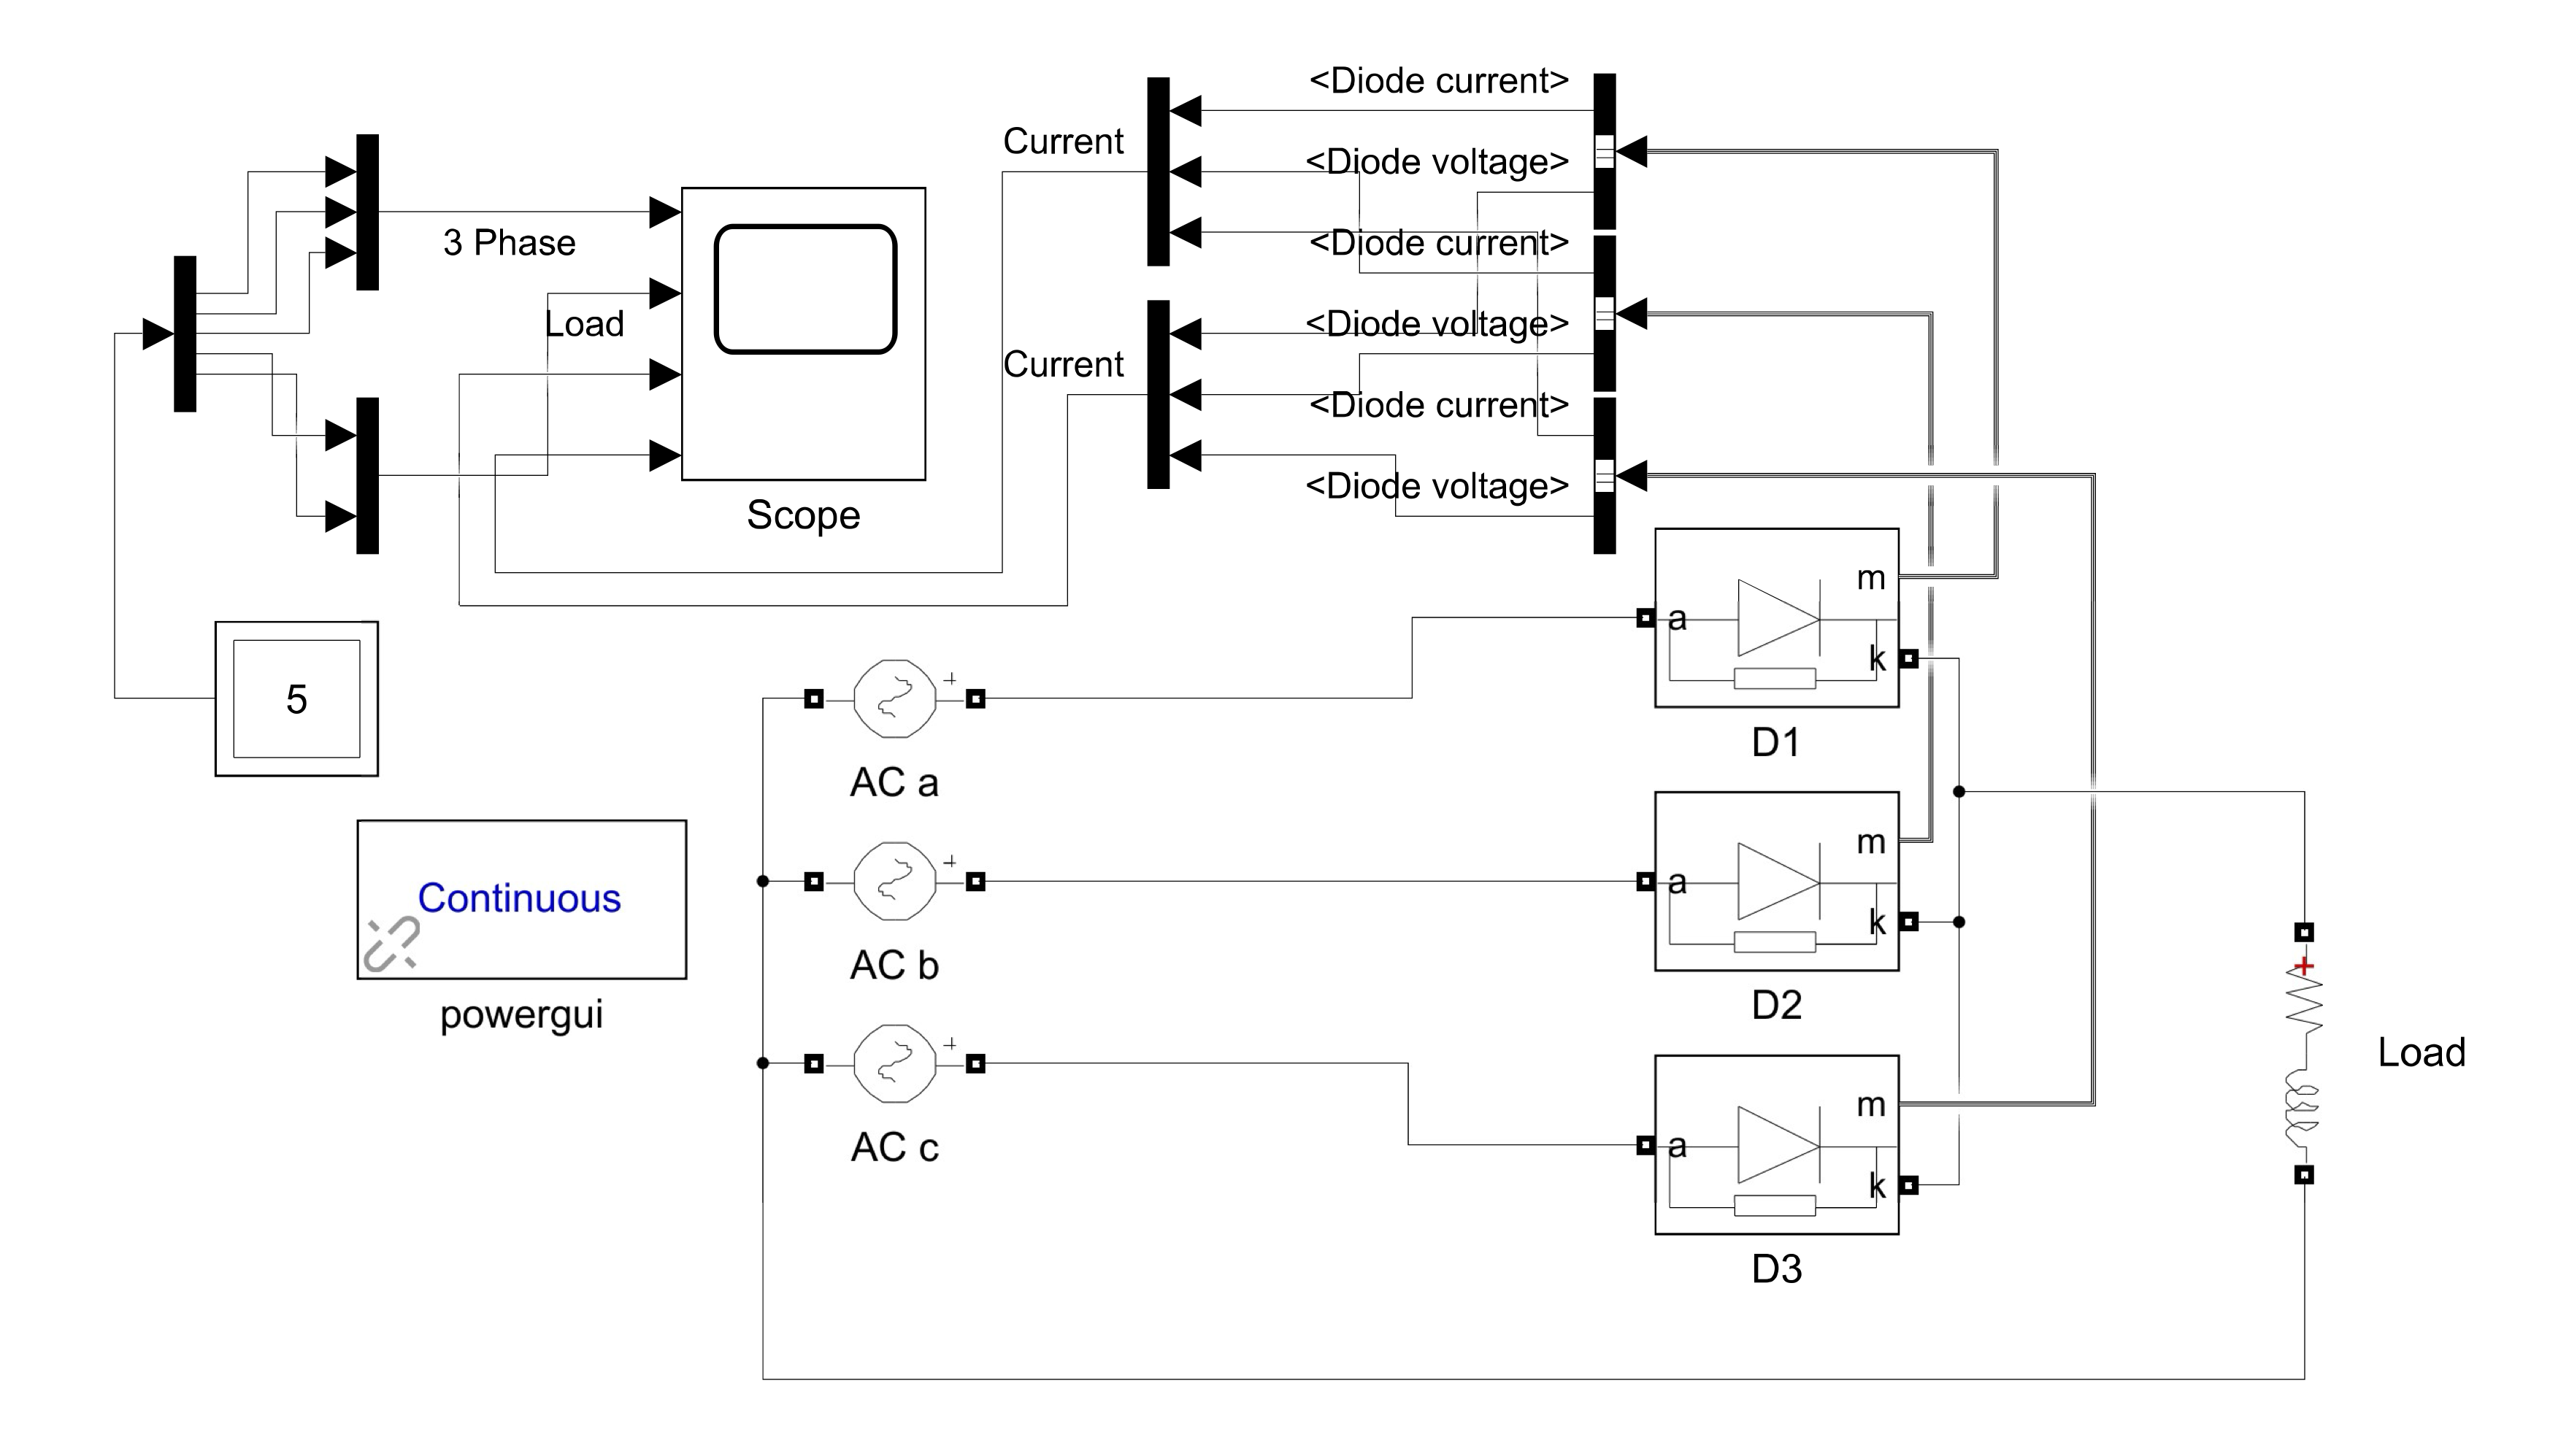
\includegraphics[width=\textwidth]{ckt.png}
    \caption{Diode with Resistive Load}
    \label{fig:dc_r_load}
\end{figure}

\section*{Observations}
\addcontentsline{toc}{section}{Observations}
\begin{itemize}
    \item The output voltage for the R load is a pulsating DC with a frequency 6 times the input AC.
    \item With gate voltage delay for the thyristor and R load, the output voltage shows a delayed conduction angle, reducing the average output.
    \item For the RL load, the output voltage is pulsating DC, with the current lagging due to inductance.
    \item Gate voltage delay for the thyristor with RL load results in a delayed conduction angle and a more pronounced current lag.
    \item MATLAB/Simulink aids in analyzing and visualizing the rectifier's performance under different loads.
\end{itemize}


\subsubsection*{Outputs}
\begin{figure}[H]
    \centering
    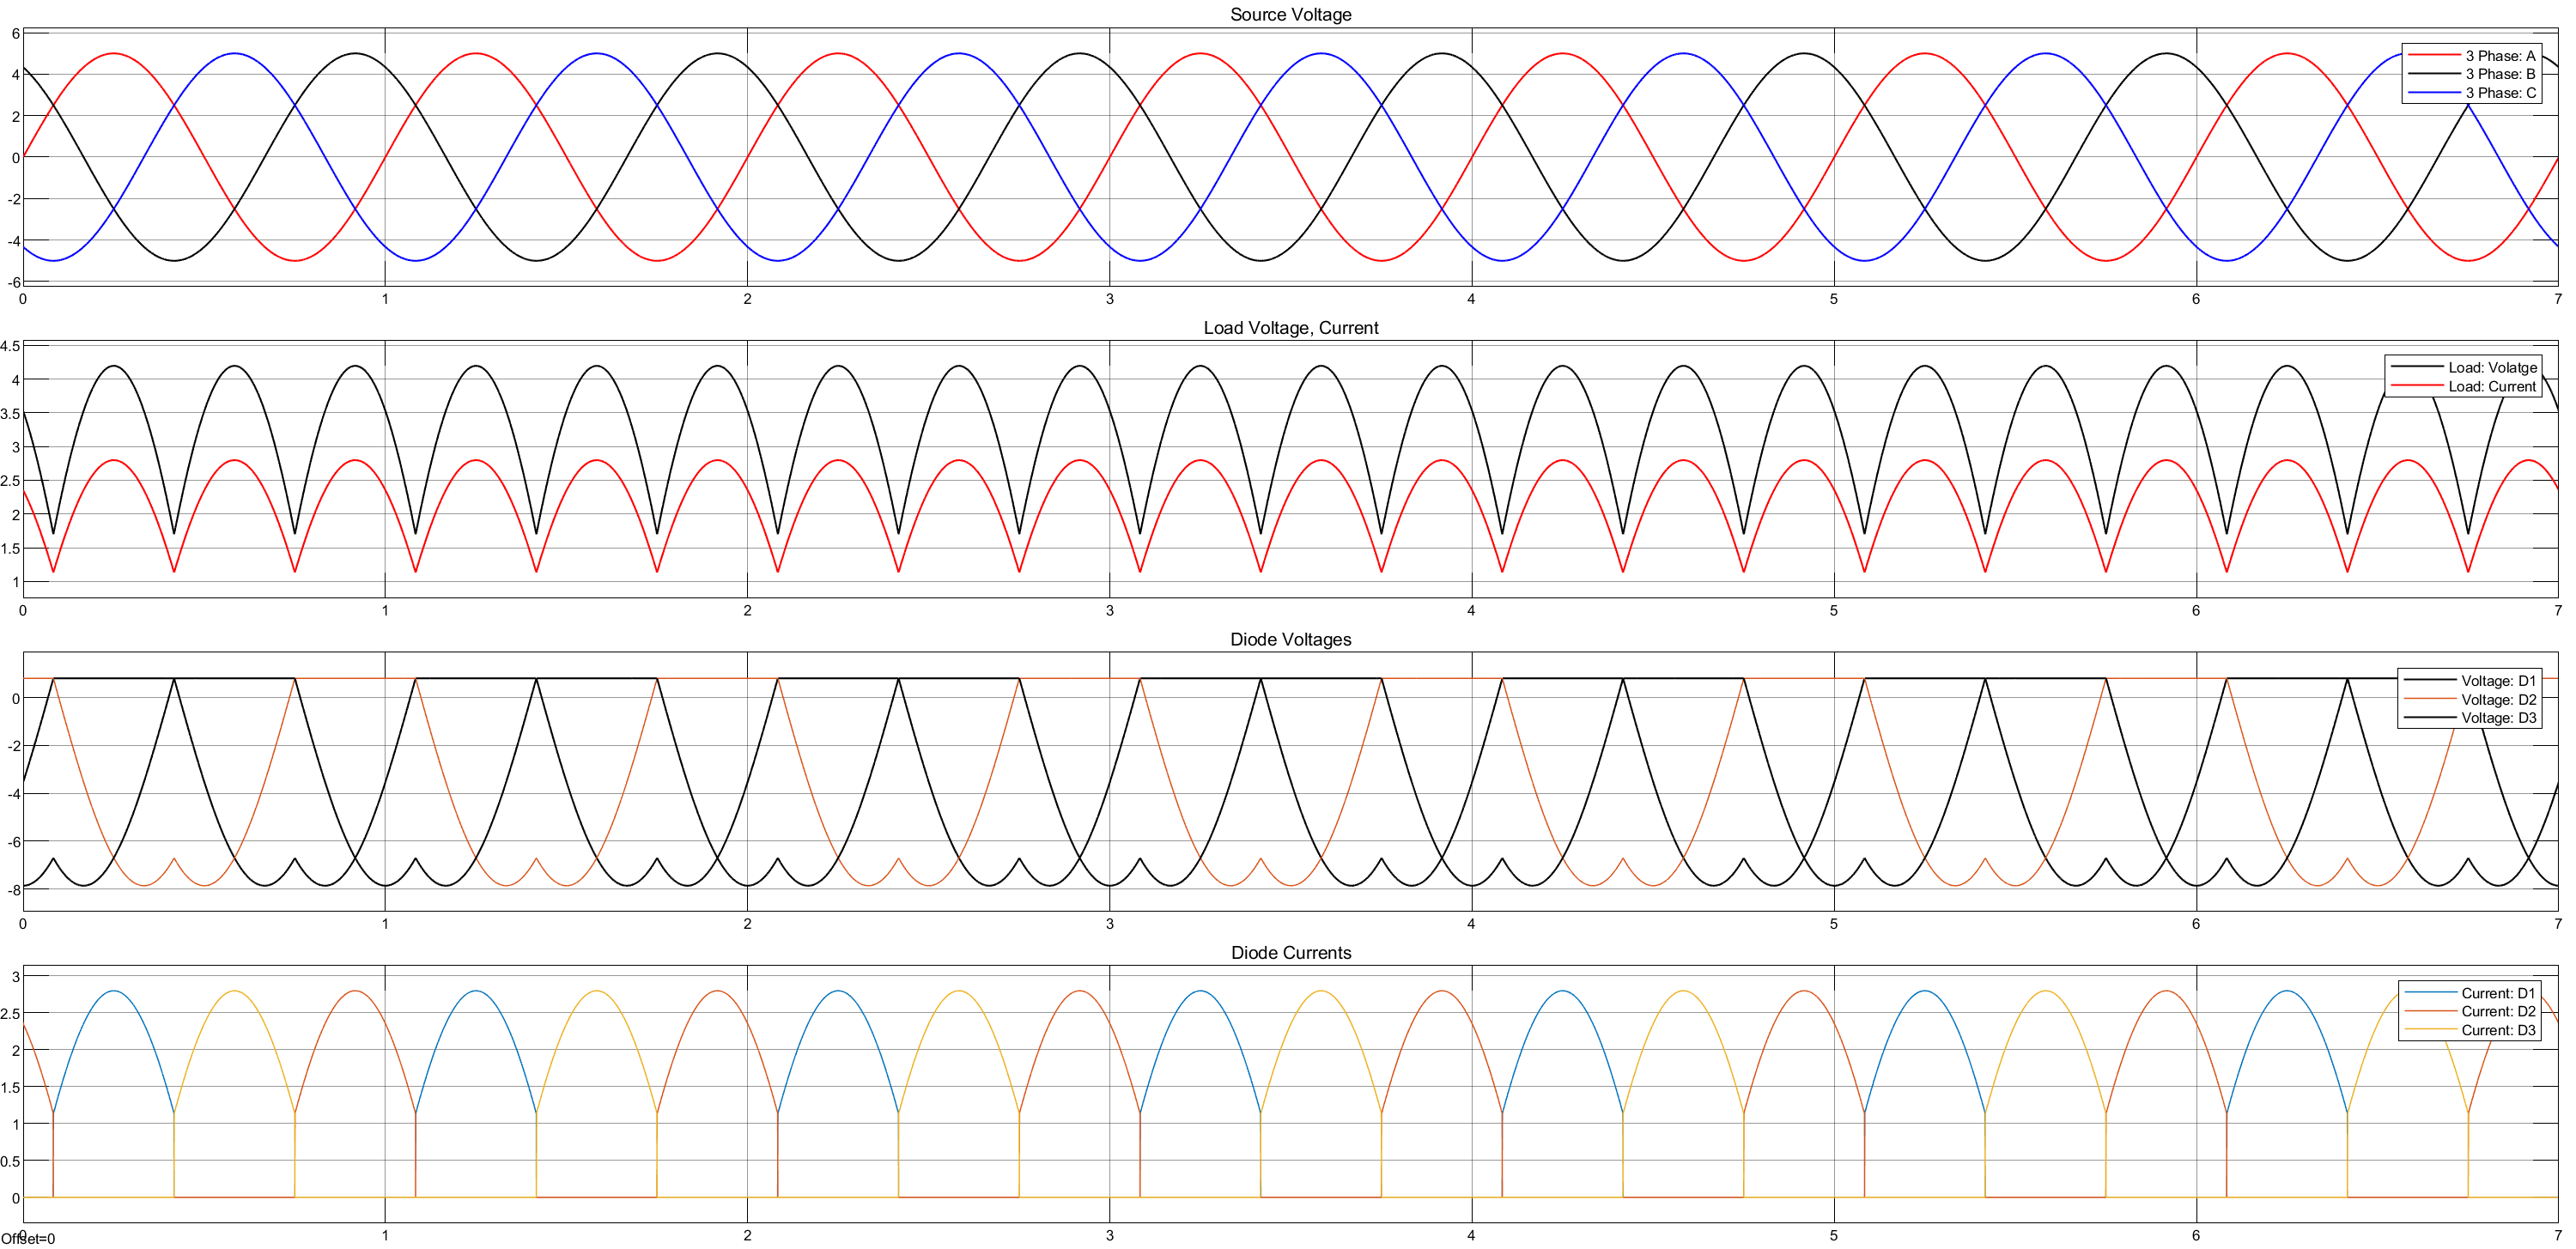
\includegraphics[width=\textwidth]{r.png}
    \caption{Simulation Output for R Load, 3 Phase Bridge Rectifier}
    \label{fig:rLoad}
\end{figure}

\begin{figure}[H]
    \centering
    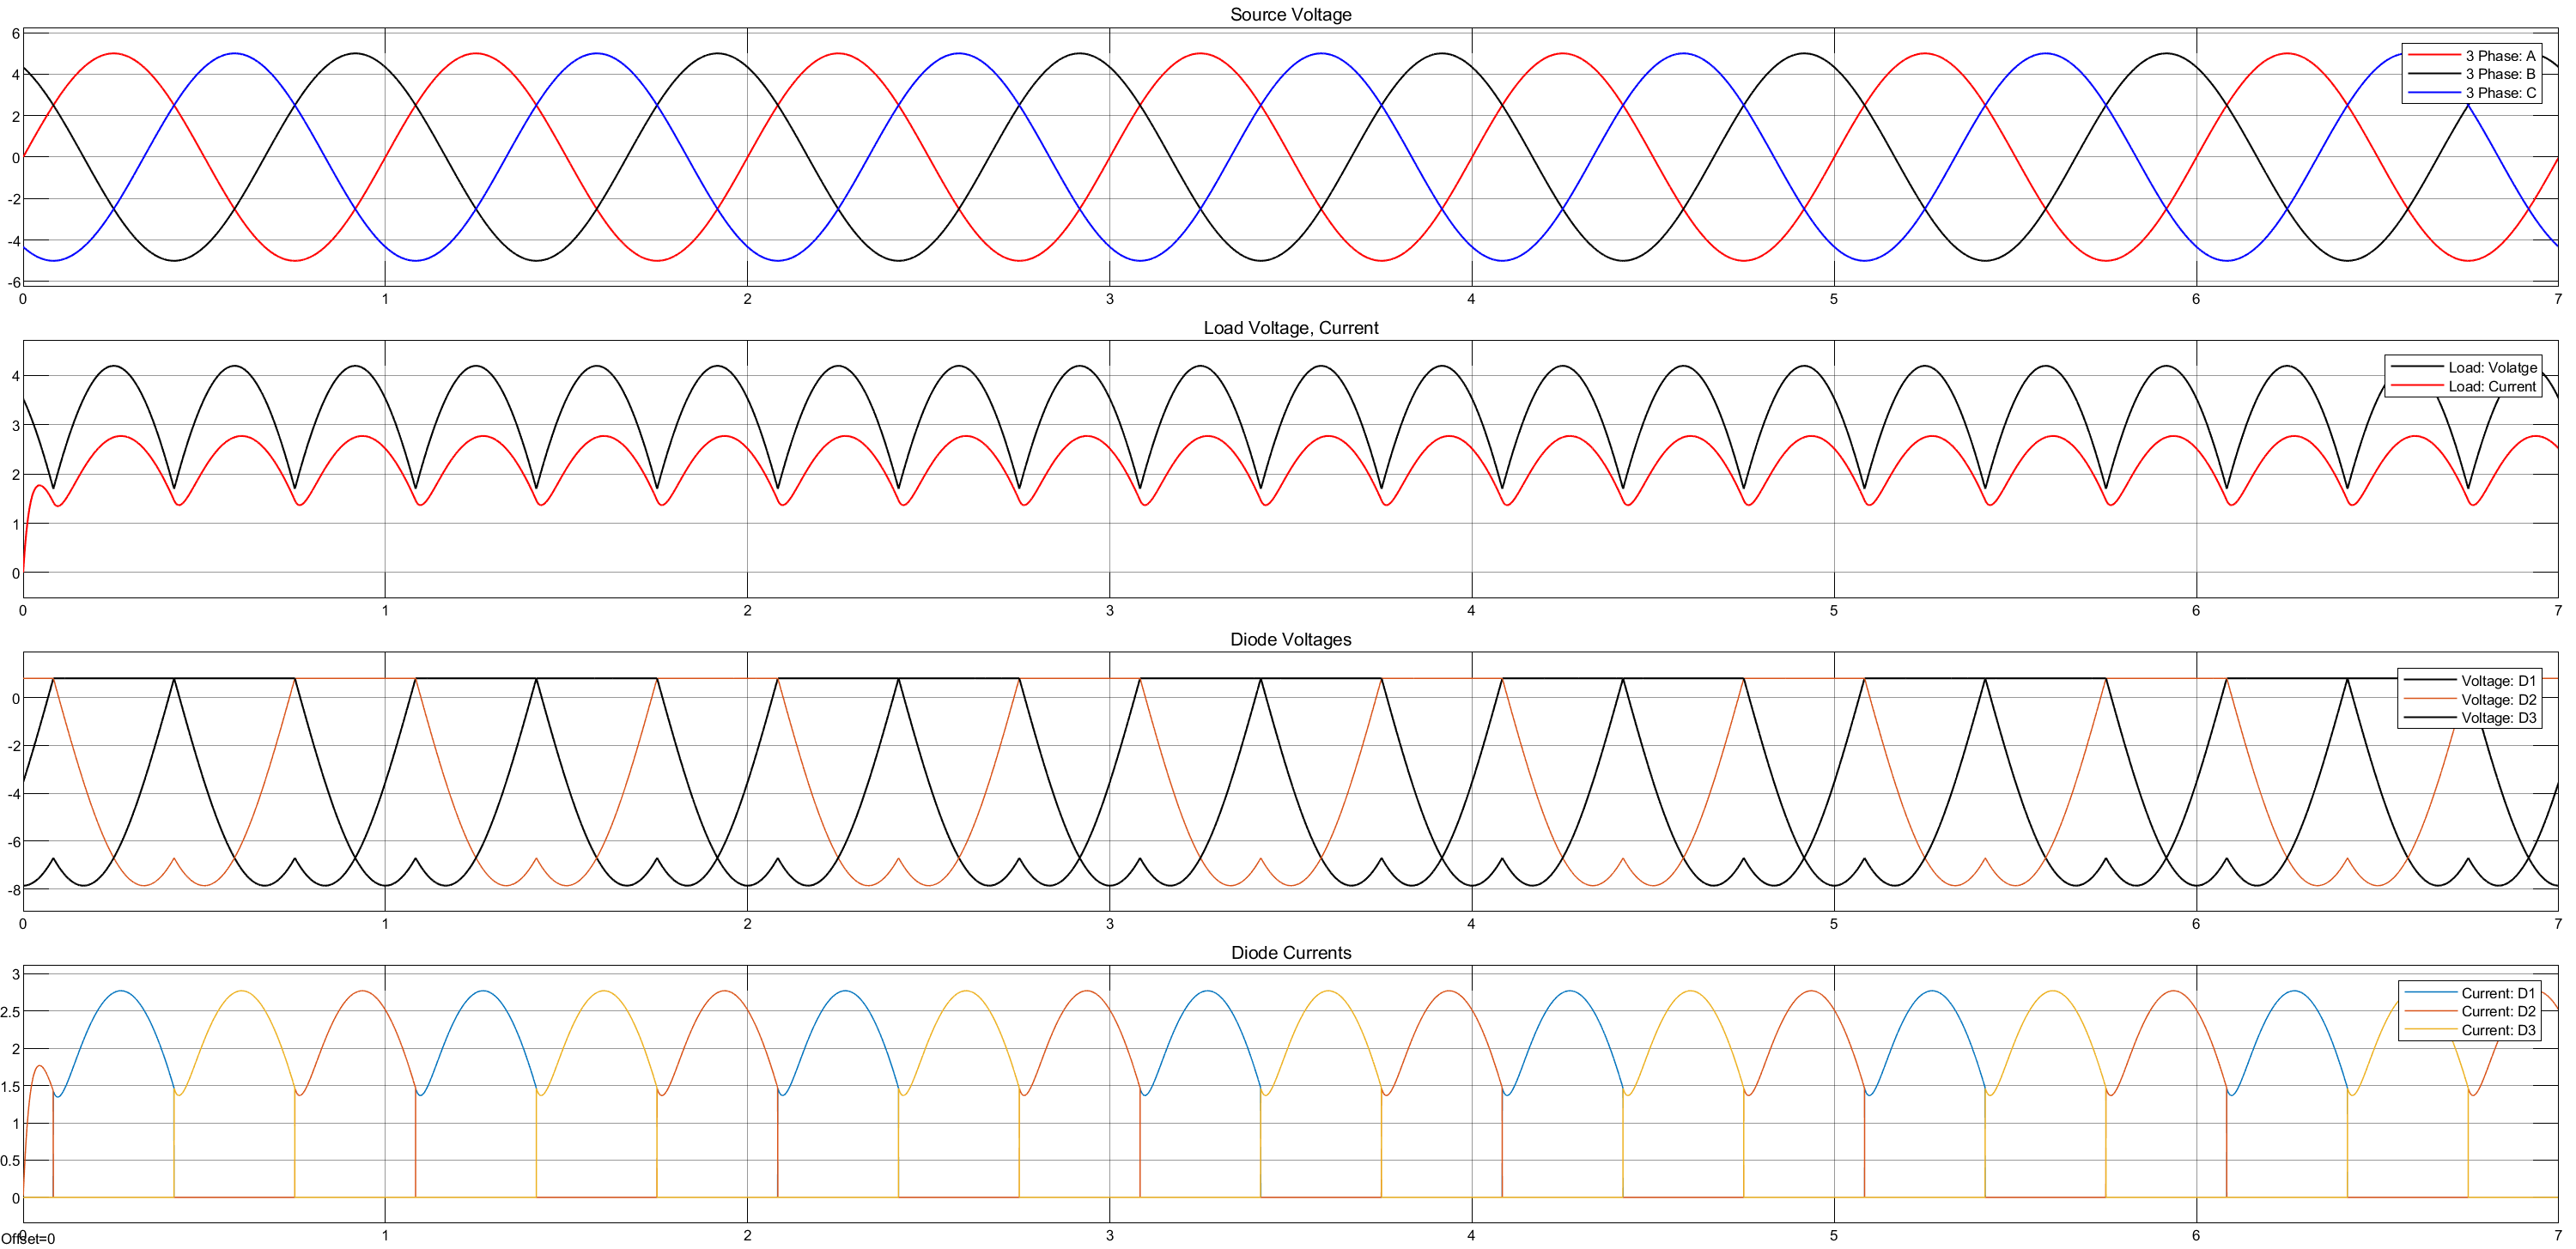
\includegraphics[width=\textwidth]{rl.png}
    \caption{Simulation Output for RL Load, 3 Phase Bridge Rectifier}
    \label{fig:rlLoad}
\end{figure}

\section*{Discussion}
\addcontentsline{toc}{section}{Discussion}
The three-phase star rectifier is a versatile circuit that can be used with different types of loads to convert AC input into DC output. By using MATLAB/Simulink, we can model the rectifier and analyze its performance under various conditions. The output voltage and current waveforms can be observed to understand the rectifier's behavior and optimize its performance for different industrial applications.

\section*{Conclusion}
\addcontentsline{toc}{section}{Conclusion}
The study of the three-phase star rectifier using diodes with R and RL loads provides valuable insights into the rectifier's behavior under different load conditions. By analyzing the output waveforms using MATLAB/Simulink, we can optimize the rectifier's performance and ensure efficient power conversion in industrial applications.

\bibliographystyle{IEEEtran}
\renewcommand{\bibname}{References}
\addcontentsline{toc}{section}{References}
\bibliography{ref}

\end{document}
